\documentclass{article}
\usepackage{amssymb}
\usepackage{amsmath}
\usepackage{geometry}
\usepackage{eufrak}
\usepackage{fixltx2e}
\usepackage{bm}
\usepackage{tikz}
\usepackage{float}
\usepackage{xcolor}
\usepackage{ulem}
\usepackage{cancel}
\usetikzlibrary{positioning}

\geometry
{
a4paper,
total={170mm,257mm},
left=20mm,
top=20mm,
}

\newcommand{\s}{\text{ }}
\newcommand{\mn}{\text{-}}
\newcommand{\la}{\langle}
\newcommand{\ra}{\rangle}

\title{Technical Summary For: \\ ``A Formalization of Membrane Systems\\ with Dynamically Evolving Structures"}
\date{\today}
\author{Ren Tristan A. de la Cruz}

% ================================================================================================ %

\begin{document}

% ================================================================================================ %

\maketitle

% ================================================================================================ %

\section{Formal Framework}

% ================================================================================================ %

\subsection{Configurations}

% ================================================================================================ %

\begin{enumerate}

% ================================================================================================ %

\item $C = \{(id_1,w_1),...,(id_j,w_j)...,(id_m,w_m)\} \subseteq (\mathbb{N} \times O^{\circ})^*$ -
      \textit{basic configuration}

\begin{figure}[H]
\begin{center}
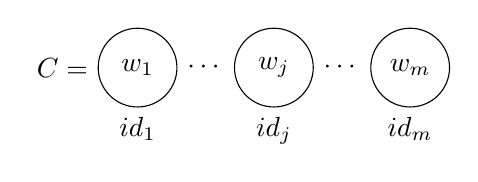
\begin{tikzpicture}
[ 
cell-a/.style={circle, draw, minimum size =  10.00mm},
text-a/.style={black}
]
\node (cell-1)    [cell-a                            ] {$w_1$};
\node (cell-1-id) [text-a, below =  00.00mm of cell-1] {$id_1$};
\node (dots-1)    [text-a, right =  00.00mm of cell-1] {$\cdots$};
\node (cell-j)    [cell-a, right =  00.00mm of dots-1] {$w_j$};
\node (cell-j-id) [text-a, below =  00.00mm of cell-j] {$id_j$};
\node (dots-2)    [text-a, right =  00.00mm of cell-j] {$\cdots$};
\node (cell-m)    [cell-a, right =  00.00mm of dots-2] {$w_m$};
\node (cell-m-id) [text-a, below =  00.00mm of cell-m] {$id_m$};
\node (C)         [text-a, left  =  00.00mm of cell-1] {$C=$};
\end{tikzpicture}
\end{center}
\end{figure}

\begin{itemize}
\item $id_j \in \mathbb{N}$ - \textit{cell id}
\item $w_j \in O^{\circ}$ - \textit{cell content}
\item $(id_j, w_j)$ - \textit{cell}
\end{itemize}

% ================================================================================================ %

\item $\mathbb{C} = \{ C \s | \s size(C) > 0\}$

\begin{itemize}
\item $size(C)$ - size of basic configuration $C$
\item $\mathbb{C}$ - set of all basic configurations with size greater than 0.
\end{itemize}

% ================================================================================================ %

\item $\mathcal{C} = (L, \rho) = (L = \{(id_1,l_1,w_1),...,(id_j,l_j,w_j),...(id_m,l_m,w_m)\}, \rho)$

\begin{figure}[H]
\begin{center}
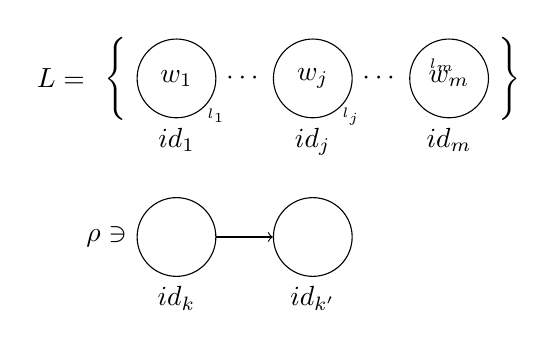
\begin{tikzpicture}
[
cell-a/.style={circle, draw, minimum size = 10mm},
text-a/.style={black}
]
\node (cell-1)     [cell-a]                                    {$w_1$};
\node (cell-1-id)  [text-a, below       =  00.00mm of cell-1]  {$id_1$};
\node (cell-1-lb)  [text-a, below right = -01.30mm of cell-1]  {\tiny $l_1$};
\node (dots-1)     [text-a, right       =  00.00mm of cell-1]  {$\cdots$};
\node (cell-j)     [cell-a, right       =  00.00mm of dots-1]  {$w_j$};
\node (cell-j-id)  [text-a, below       =  00.00mm of cell-j]  {$id_j$};
\node (cell-j-lb)  [text-a, below right = -01.50mm of cell-j]  {\tiny $l_j$};
\node (dots-2)     [text-a, right       =  00.00mm of cell-j]  {$\cdots$};
\node (cell-m)     [cell-a, right       =  00.00mm of dots-2]  {$w_m$};
\node (cell-m-id)  [text-a, below       =  00.00mm of cell-m]  {$id_m$};
\node (cell-m-lb)  [text-a, below right = -10.30mm of cell-m]  {\tiny $l_m$};
\node (brac-1)     [text-a, left        =  00.00mm of cell-1]  {$\Bigg \{$};
\node (brac-2)     [text-a, right       =  00.00mm of cell-m]  {$\Bigg \}$};
\node (L)          [text-a, left        =  00.00mm of brac-1]  {$L=$};
\node (cell-k)     [cell-a, below       =  10.00mm of cell-1]  {};
\node (cell-k-id)  [text-a, below       =  00.00mm of cell-k]  {$id_k$};
\node (cell-k')    [cell-a, below       =  10.00mm of cell-j]  {};
\node (cell-k'-id) [text-a, below       =  00.00mm of cell-k'] {$id_{k'}$};
\node (rho)        [text-a, left        =  00.00mm of cell-k]  {$\rho \ni$};
\draw [->] (cell-k) -- (cell-k');
\end{tikzpicture}
\end{center}
\end{figure}

% ================================================================================================ %

\begin{itemize}
\item $id_j \in \mathbb{N}$ - \textit{id}
\item $w_j \in O^{\circ}$ - \textit{multiset} over $O$
\item $l_j \in Lab$ - \textit{label} 
\item $(id_j,l_j,w_j)$ - \textit{labelled cell}
\item $L \in (\mathbb{N} \times Lab \times O^{\circ})^*$ - list of labelled cells
\item $\rho \subseteq \mathbb{N} \times \mathbb{N}$ - \textit{relations} between cells (ids)
\item $\mathcal{C} = (L, \rho)$ - \textit{configuration} 
\item $\mathcal{C}_L = L$ and $\mathcal{C}_\rho = \rho$.
\item $\overline{\mathcal{C}}_L \in \mathbb{C}$ -  \textit{projection} of $\mathcal{C}_L$ 
      as basic configuration.

\begin{figure}[H]
\begin{center}
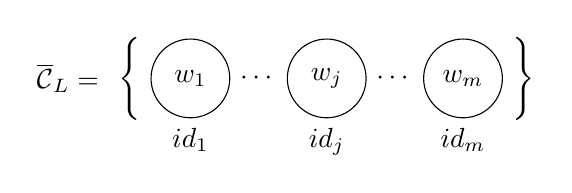
\begin{tikzpicture}
[ 
cell-a/.style={circle, draw, minimum size = 10mm},
text-a/.style={black}
]
\node (cell-1)     [cell-a]                              {$w_1$};
\node (cell-1-d)   [text-a, below =  00.00mm of cell-1]  {$id_1$};
\node (dots-1)     [text-a, right =  00.00mm of cell-1]  {$\cdots$};
\node (cell-j)     [cell-a, right =  00.00mm of dots-1]  {$w_j$};
\node (cell-j-id)  [text-a, below =  00.00mm of cell-j]  {$id_j$};
\node (dots-2)     [text-a, right =  00.00mm of cell-j]  {$\cdots$};
\node (cell-m)     [cell-a, right =  00.00mm of dots-2]  {$w_m$};
\node (cell-m-id)  [text-a, below =  00.00mm of cell-m]  {$id_m$};
\node (brac-1)     [text-a, left  =  00.00mm of cell-1]  {$\Bigg \{$};
\node (brac-2)     [text-a, right =  00.00mm of cell-m]  {$\Bigg \}$};
\node (CL)         [text-a, left  =  00.00mm of brac-1]  {$\overline{\mathcal{C}}_L =$};
\end{tikzpicture}
\end{center}
\end{figure}
\end{itemize}

% ================================================================================================ %

\item $\mathfrak{C} = \{\mathcal{C} \s | \s \mathcal{C} = (L, \rho)\}$

\begin{itemize}
\item $\mathfrak{C}$ is the set of all possible configurations.
\end{itemize}

% ================================================================================================ %

\end{enumerate}

% ================================================================================================ %

\subsection{Components of a Rule}
\begin{enumerate}
\setcounter{enumi}{-1}

% ================================================================================================ %

\item $r = (Labels, \rho, Perm, For, Rewrite, Label\mn Rename, Delete, Delete\mn and\mn Move, 
          Generate, Generate\mn and\mn Copy,\\ Change\mn Relation)$
         
\begin{itemize}
\item $r$ is a rule.
\end{itemize}

% ================================================================================================ %

\item $Labels(r) = (l_1,...,l_j....,l_k) \in Lab^k$ 

\begin{figure}[H]
\begin{center}
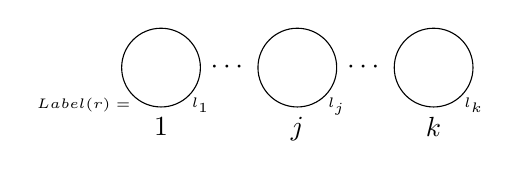
\begin{tikzpicture}
[ 
cell-a/.style={circle, draw, minimum size = 10mm},
text-a/.style={black}
]
\node (cell-1)     [cell-a]                                  {$ $};
\node (cell-1-id)  [text-a, below       =  0.0mm of cell-1]  {$1$};
\node (cell-1-lb)  [text-a, below right = -1.3mm of cell-1]  {\tiny $l_1$};
\node (dots-1)     [text-a, right       =  0.0mm of cell-1]  {$\cdots$};
\node (cell-j)     [cell-a, right       =  0.0mm of dots-1]  {$ $};
\node (cell-j-id)  [text-a, below       =  0.0mm of cell-j]  {$j$};
\node (cell-j-lb)  [text-a, below right = -1.3mm of cell-j]  {\tiny $l_j$};
\node (dots-2)     [text-a, right       =  0.0mm of cell-j]  {$\cdots$};
\node (cell-k)     [cell-a, right       =  0.0mm of dots-2]  {$ $};
\node (cell-k-id)  [text-a, below       =  0.0mm of cell-k]  {$k$};
\node (cell-k-lb)  [text-a, below right = -1.3mm of cell-k]  {\tiny $l_k$};
\node (Lab)        [text-a, below left  = -1.3mm of cell-1]  {\tiny $Label(r)=$};
\end{tikzpicture}
\end{center}
\end{figure}

% ================================================================================================ %

\item $\rho(r) \subseteq \mathbb{N}_k \times \mathbb{N}_k$

\begin{itemize}
\item $\mathbb{N}_k = \{1,...,j,...,k\}$
\end{itemize}

% ================================================================================================ %

\item $Perm(r) =\{P_1,...,P_{j'},...,P_{\overline{p}}\}\subseteq \mathbb{C}_k$

\begin{figure}[H]
\begin{center}
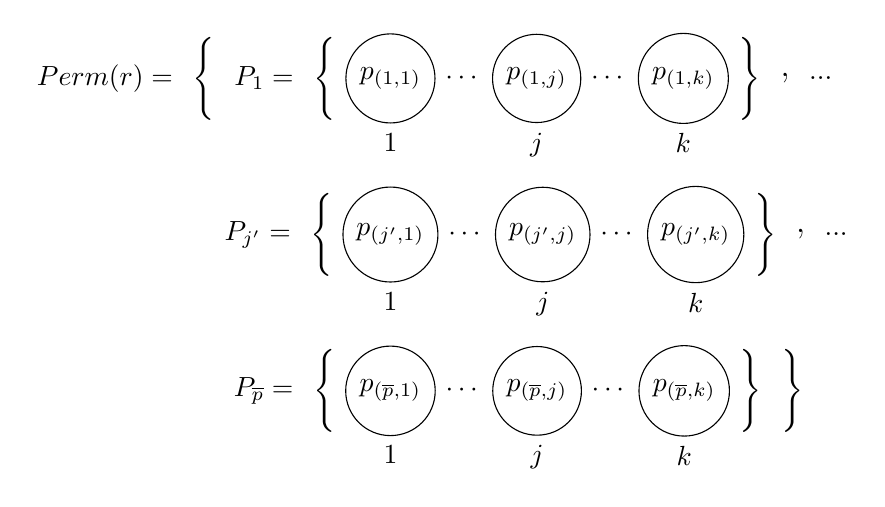
\begin{tikzpicture}
[
cell-a/.style={circle, draw, minimum size = 10mm},
cell-b/.style={circle, draw, minimum size = 10mm, dotted},
text-a/.style={black}
]
\node (cell-11)    [cell-a]                              {$p_{(1,1)}$};
\node (cell-11-id) [text-a, below =  00.00mm of cell-11] {$1$};
\node (dots-1)     [text-a, right =  00.00mm of cell-11] {$\cdots$};
\node (cell-1j)    [cell-a, right =  00.00mm of dots-1 ] {$p_{(1,j)}$};
\node (cell-1j-id) [text-a, below =  00.00mm of cell-1j] {$j$};
\node (dots-2)     [text-a, right =  00.00mm of cell-1j] {$\cdots$};
\node (cell-1k)    [cell-a, right =  00.00mm of dots-2 ] {$p_{(1,k)}$};
\node (cell-1k-id) [text-a, below =  00.00mm of cell-1k] {$k$};
\node (brac-11)    [text-a, left  =  00.00mm of cell-11] {$\Bigg\{$};
\node (brac-12)    [text-a, right =  00.00mm of cell-1k] {$\Bigg\}$};
\node (P1)         [text-a, left  =  00.00mm of brac-11] {$P_1=$};
\node (coma1)      [text-a, right =  00.00mm of brac-12] {\large $,$};
\node (brac-01)    [text-a, left  =  00.00mm of P1     ] {$\Bigg\{$};
\node (dots-0')    [text-a, right =  00.00mm of coma1  ] {$...$};
\node (cell-j1)    [cell-a, below =  08.00mm of cell-11] {$p_{(j',1)}$};
\node (cell-j1-id) [text-a, below =  00.00mm of cell-j1] {$1$};
\node (dots-3)     [text-a, right =  00.00mm of cell-j1] {$\cdots$};
\node (cell-jj)    [cell-a, right =  00.00mm of dots-3 ] {$p_{(j',j)}$};
\node (cell-jj-id) [text-a, below =  00.00mm of cell-jj] {$j$};
\node (dots-3)     [text-a, right =  00.00mm of cell-jj] {$\cdots$};
\node (cell-jk)    [cell-a, right =  00.00mm of dots-3 ] {$p_{(j',k)}$};
\node (cell-jk-id) [text-a, below =  00.00mm of cell-jk] {$k$};
\node (brac-j1)    [text-a, left  =  00.00mm of cell-j1] {$\Bigg\{$};
\node (brac-j2)    [text-a, right =  00.00mm of cell-jk] {$\Bigg\}$};
\node (PJ)         [text-a, left  =  00.00mm of brac-j1] {$P_{j'}=$};
\node (coma2)      [text-a, right =  00.00mm of brac-j2] {\large $,$};
\node (dots-1')    [text-a, right =  00.00mm of coma2  ] {$...$};
\node (cell-p1)    [cell-a, below =  08.00mm of cell-j1] {$p_{(\overline{p},1)}$};
\node (cell-p1-d)  [text-a, below =  00.00mm of cell-p1] {$1$};
\node (dots-4)     [text-a, right =  00.00mm of cell-p1] {$\cdots$};
\node (cell-pj)    [cell-a, right =  00.00mm of dots-4 ] {$p_{(\overline{p},j)}$};
\node (cell-pj-id) [text-a, below =  00.00mm of cell-pj] {$j$};
\node (dots-4)     [text-a, right =  00.00mm of cell-pj] {$\cdots$};
\node (cell-pk)    [cell-a, right =  00.00mm of dots-4 ] {$p_{(\overline{p},k)}$};
\node (cell-pk-id) [text-a, below =  00.00mm of cell-pk] {$k$};
\node (brac-p1)    [text-a, left  =  00.00mm of cell-p1] {$\Bigg\{$};
\node (brac-p2)    [text-a, right =  00.00mm of cell-pk] {$\Bigg\}$};
\node (PP)         [text-a, left  =  00.00mm of brac-p1] {$P_{\overline{p}}=$};
\node (brac-02)    [text-a, right =  00.00mm of brac-p2] {$\Bigg\}$};
\node (Perm)       [text-a, left  =  00.00mm of brac-01] {$Perm(r)=$};
\end{tikzpicture}
\end{center}
\end{figure}

\begin{itemize}
\item $\mathbb{C}_k \subseteq \mathbb{C}$ -  \textit{basic configurations} with cell ids in
      $\mathbb{N}_k$.
\item $p_{(j',j)} \in O^{\circ}$ 
\end{itemize}

% ================================================================================================ %

\item $For(r) =\{F_1,...,F_{j'},...,F_{\overline{f}}\}\subseteq \mathbb{C}_k$

\begin{figure}[H]
\begin{center}
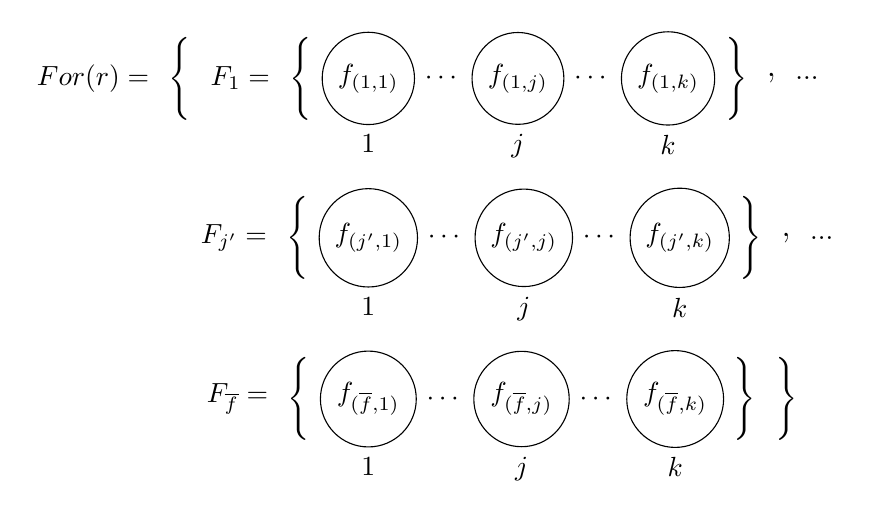
\begin{tikzpicture}
[
cell-a/.style={circle, draw, minimum size = 10mm},
cell-b/.style={circle, draw, minimum size = 10mm, dotted},
text-a/.style={black}
]
\node (cell-11)    [cell-a]                              {$f_{(1,1)}$};
\node (cell-11-id) [text-a, below =  00.00mm of cell-11] {$1$};
\node (dots-1)     [text-a, right =  00.00mm of cell-11] {$\cdots$};
\node (cell-1j)    [cell-a, right =  00.00mm of dots-1 ] {$f_{(1,j)}$};
\node (cell-1j-id) [text-a, below =  00.00mm of cell-1j] {$j$};
\node (dots-2)     [text-a, right =  00.00mm of cell-1j] {$\cdots$};
\node (cell-1k)    [cell-a, right =  00.00mm of dots-2 ] {$f_{(1,k)}$};
\node (cell-1k-id) [text-a, below =  00.00mm of cell-1k] {$k$};
\node (brac-11)    [text-a, left  =  00.00mm of cell-11] {$\Bigg\{$};
\node (brac-12)    [text-a, right =  00.00mm of cell-1k] {$\Bigg\}$};
\node (F1)         [text-a, left  =  00.00mm of brac-11] {$F_1=$};
\node (coma1)      [text-a, right =  00.00mm of brac-12] {\large $,$};
\node (brac-01)    [text-a, left  =  00.00mm of F1     ] {$\Bigg\{$};
\node (dots-0')    [text-a, right =  00.00mm of coma1  ] {$...$};
\node (cell-j1)    [cell-a, below =  08.00mm of cell-11] {$f_{(j',1)}$};
\node (cell-j1-id) [text-a, below =  00.00mm of cell-j1] {$1$};
\node (dots-3)     [text-a, right =  00.00mm of cell-j1] {$\cdots$};
\node (cell-jj)    [cell-a, right =  00.00mm of dots-3 ] {$f_{(j',j)}$};
\node (cell-jj-id) [text-a, below =  00.00mm of cell-jj] {$j$};
\node (dots-3)     [text-a, right =  00.00mm of cell-jj] {$\cdots$};
\node (cell-jk)    [cell-a, right =  00.00mm of dots-3 ] {$f_{(j',k)}$};
\node (cell-jk-id) [text-a, below =  00.00mm of cell-jk] {$k$};
\node (brac-j1)    [text-a, left  =  00.00mm of cell-j1] {$\Bigg\{$};
\node (brac-j2)    [text-a, right =  00.00mm of cell-jk] {$\Bigg\}$};
\node (FJ)         [text-a, left  =  00.00mm of brac-j1] {$F_{j'}=$};
\node (coma2)      [text-a, right =  00.00mm of brac-j2] {\large $,$};
\node (dots-1')    [text-a, right =  00.00mm of coma2  ] {$...$};
\node (cell-f1)    [cell-a, below =  08.00mm of cell-j1] {$f_{(\overline{f},1)}$};
\node (cell-f1-d)  [text-a, below =  00.00mm of cell-f1] {$1$};
\node (dots-4)     [text-a, right =  00.00mm of cell-f1] {$\cdots$};
\node (cell-fj)    [cell-a, right =  00.00mm of dots-4 ] {$f_{(\overline{f},j)}$};
\node (cell-fj-id) [text-a, below =  00.00mm of cell-fj] {$j$};
\node (dots-4)     [text-a, right =  00.00mm of cell-fj] {$\cdots$};
\node (cell-fk)    [cell-a, right =  00.00mm of dots-4 ] {$f_{(\overline{f},k)}$};
\node (cell-fk-id) [text-a, below =  00.00mm of cell-fk] {$k$};
\node (brac-f1)    [text-a, left  =  00.00mm of cell-f1] {$\Bigg\{$};
\node (brac-f2)    [text-a, right =  00.00mm of cell-fk] {$\Bigg\}$};
\node (FF)         [text-a, left  =  00.00mm of brac-f1] {$F_{\overline{f}}=$};
\node (brac-02)    [text-a, right =  00.00mm of brac-f2] {$\Bigg\}$};
\node (For)        [text-a, left  =  00.00mm of brac-01] {$For(r)=$};
\end{tikzpicture}
\end{center}
\end{figure}

\begin{itemize}
\item $f_{(j',j)} \in O^{\circ}$ 
\end{itemize}

% ================================================================================================ %

\item $Rewrite(r) = U \rightarrow V$
\begin{itemize}
\item $U, V \in \mathbb{C}_k$
\item $Rewrite(r)$ is a general rewriting rule, rewriting a finite basic configuration $U$ to another finite basic configuration $V$.
\end{itemize}

% ================================================================================================ %

\item $Label\mn Rename(r)=\{...,(i,l'),...\} \in (\mathbb{N}_k \times Lab)^*$

\begin{figure}[H]
\begin{center}
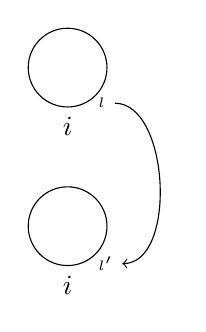
\begin{tikzpicture}
[ 
cell-a/.style={circle, draw, minimum size = 10mm},
text-a/.style={}
]
\node (cell-i)     [cell-a]                                  { };
\node (cell-i-id)  [text-a, below       =  0.0mm of cell-i ] {$i$};
\node (cell-i-lb)  [text-a, below right = -1.3mm of cell-i ] {\tiny $l$};
\node (cell-i2)    [cell-a, below       =  1.0cm of cell-i ] { };
\node (cell-i2-id) [text-a, below       =  0.0mm of cell-i2] {$i$};
\node (cell-i2-lb) [text-a, below right = -1.3mm of cell-i2] {\tiny $l'$};
\draw [->] (cell-i-lb.east) .. controls +(right:07.00mm) and +(right:07.00mm) .. (cell-i2-lb.east);
\end{tikzpicture}
\end{center}
\end{figure}

\begin{itemize}
\item $i \in \mathbb{N}_k$ - \textit{id}
\item $l' \in Lab$ - new label
\end{itemize}

% ================================================================================================ %

\item $Delete(r)=\{...,j,...\}\in \mathbb{N}_k^*$

\begin{figure}[H]
\begin{center}
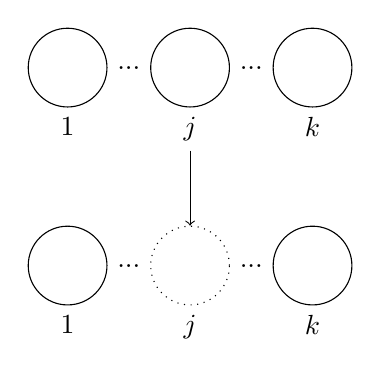
\begin{tikzpicture}
[ 
cell-a/.style={circle, draw, minimum size = 10mm},
cell-b/.style={circle, draw, minimum size = 10mm, dotted},
text-a/.style={}
]
\node (cell-1)     [cell-a]                           {};
\node (cell-1-id)  [text-a, below = 0.0cm of cell-1 ] {$1$};
\node (dots-1)     [text-a, right = 0.0cm of cell-1 ] {$...$};
\node (cell-j)     [cell-a, right = 0.0cm of dots-1 ] {};
\node (cell-j-id)  [text-a, below = 0.0cm of cell-j ] {$j$};
\node (dots-2)     [text-a, right = 0.0cm of cell-j ] {$...$};
\node (cell-k)     [cell-a, right = 0.0cm of dots-2 ] {};
\node (cell-k-id)  [text-a, below = 0.0cm of cell-k ] {$k$};
\node (cell-12)    [cell-a, below = 1.5cm of cell-1 ] {};
\node (cell-12-id) [text-a, below = 0.0cm of cell-12] {$1$};
\node (dots-3)     [text-a, right = 0.0cm of cell-12] {$...$};
\node (cell-j2)    [cell-b, right = 0.0cm of dots-3 ] {};
\node (cell-j2-id) [text-a, below = 0.0cm of cell-j2] {$j$};
\node (dots-4)     [text-a, right = 0.0cm of cell-j2] {$...$};
\node (cell-k2)    [cell-a, right = 0.0cm of dots-4 ] {};
\node (cell-k2-id) [text-a, below = 0.0cm of cell-k2] {$k$};
\draw [ ->] (cell-j-id) -- (cell-j2);
\end{tikzpicture}
\end{center}
\end{figure}

\begin{itemize}
\item $j$ - \textit{id} of cell to be deleted
\end{itemize}

% ================================================================================================ %

\item $Delete\mn Move(r) \in (\mathbb{N}_k \times \mathbb{N}_k)^*$

\begin{figure}[H]
\begin{center}
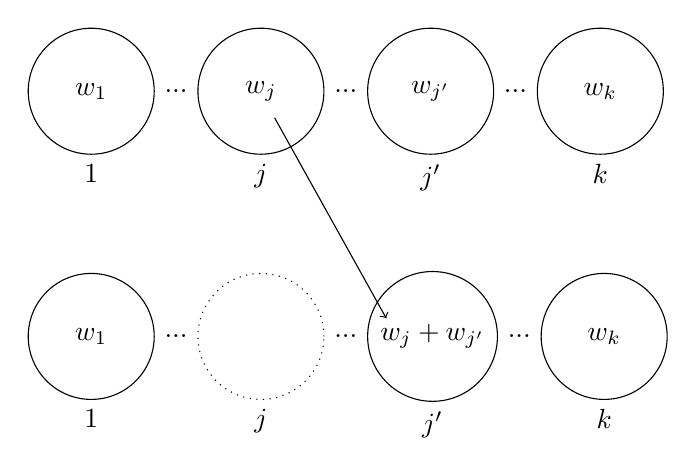
\begin{tikzpicture}
[scale=1.0, 
cell-a/.style={circle, draw, minimum size = 16mm},
cell-b/.style={circle, draw, dotted,minimum size = 16mm},
text-a/.style={},]
%\draw [dotted, step=1.0] (-5,-5) grid (5,5); \draw [->] (0,0) -- (0,-5); \draw [->] (0,0) -- (5,0);
\node (cell-1)  [cell-a]                       {$w_1$};
\node (cell-1-id)  [text-a, below = 0.0cm of cell-1]   {$1$};
\node (dots-1)  [text-a, right = 0.0cm of cell-1]   {$...$};
\node (cell-j)  [cell-a,right = 0.0cm of dots-1]   {$w_j$};
\node (ij)  [text-a, below = 0.0cm of cell-j]   {$j$};
\node (dj)  [text-a, right = 0.0cm of cell-j]   {$...$};
\node (cell-j') [cell-a,right = 0.0cm of dj]   {$w_{j'}$};
\node (ij') [text-a, below = 0.0cm of cell-j']  {$j'$};
\node (dj') [text-a, right = 0.0cm of cell-j']  {$...$};
\node (cell-k)  [cell-a,right = 0.0cm of dj']  {$w_k$};
\node (cell-k-id)  [text-a, below = 0.0cm of cell-k]   {$k$};
\node (cell-12) [cell-a,below = 1.5cm of cell-1]   {$w_1$};
\node (cell-12-id) [text-a, below = 0.0cm of cell-12]  {$1$};
\node (dots-12) [text-a, right = 0.0cm of cell-12]  {$...$};
\node (cell-j2) [cell-b,right = 0.0cm of dots-12]  {$ $};
\node (ij2) [text-a, below = 0.0cm of cell-j2]  {${j}$};
\node (dj2) [text-a, right = 0.0cm of cell-j2]  {$...$};
\node (cell-j2')[cell-a,right = 0.0cm of dj2]  {$w_j + w_{j'}$};
\node (ij2')[text-a, below = 0.0cm of cell-j2'] {$j'$};
\node (dj2')[text-a, right = 0.0cm of cell-j2'] {$...$};
\node (cell-k2) [cell-a,right = 0.0cm of dj2'] {$w_k$};
\node (cell-k-id2) [text-a, below = 0.0cm of cell-k2]  {$k$};
\node (basj) [circle, minimum size=0.7cm] at (cell-j.base) {};
\node (bsj') [rectangle, minimum height = 7mm] at (cell-j2'.north west) {};
\draw [ ->] (basj) -- (bsj'.south);
\end{tikzpicture}
\end{center}
\end{figure}

\begin{itemize}
\item $(j,j')$ - \textit{pair of ids}
\item $j$ - \textit{id} of cell to be deleted
\item $j'$ - \textit{id} of cell to receive the multiset
\item $Delete\mn Move(r)$- \textit{list of pairs} of ids
\end{itemize}

% ================================================================================================ %

\item $Generate(r) =\{...,(j',h, u),...\} \in (\mathbb{N}' \times Lab \times O^{\circ})^*$

\begin{figure}[H]
\begin{center}
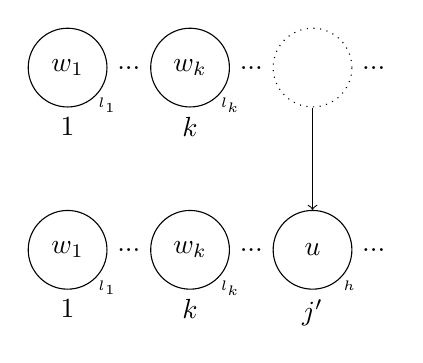
\begin{tikzpicture}
[
cell-a/.style={circle, draw, minimum size = 10mm},
cell-b/.style={circle, draw, dotted, minimum size = 10mm},
text-a/.style={}
]

\node (cell-1)     [cell-a]                                  {$w_1$};
\node (cell-1-id)  [text-a, below       =  0.0cm of cell-1]  {$1$};
\node (cell-1-lb)  [text-a, below right = -1.3mm of cell-1]  {\tiny $l_1$};
\node (dots-1)     [text-a, right       =  0.0mm of cell-1]  {$...$};
\node (cell-k)     [cell-a, right       =  0.0mm of dots-1]  {$w_k$};
\node (cell-k-id)  [text-a, below       =  0.0cm of cell-k]  {$k$};
\node (cell-k-lb)  [text-a, below right = -1.3mm of cell-k]  {\tiny $l_k$};
\node (dots-2)     [text-a, right       =  0.0mm of cell-k]  {$...$};
\node (cell-vt)    [cell-b, right       =  0.0mm of dots-2]  {};
\node (dots-3)     [text-a, right       =  0.0mm of cell-vt] {$...$};
\node (cell-12)    [cell-a, below       =  1.3cm of cell-1]  {$w_1$};
\node (cell-12-id) [text-a, below       =  0.0cm of cell-12] {$1$};
\node (l1)         [text-a, below right = -1.3mm of cell-12] {\tiny $l_1$};
\node (dots-12)    [text-a, right       =  0.0mm of cell-12] {$...$};
\node (cell-k2)    [cell-a, right       =  0.0mm of dots-12] {$w_k$};
\node (cell-k2-id) [text-a, below       =  0.0cm of cell-k2] {$k$};
\node (cell-k2-lb) [text-a, below right = -1.3mm of cell-k2] {\tiny $l_k$};
\node (dots-22)    [text-a, right       =  0.0mm of cell-k2] {$...$};
\node (cell-j')    [cell-a, right       =  0.0mm of dots-22] {$u$};
\node (cell-j'-id) [text-a, below       =  0.0cm of cell-j'] {$j'$};
\node (cell-j'-lb) [text-a, below right = -1.3mm of cell-j'] {\tiny $h$};
\node (dots-23)    [text-a, right       =  0.0mm of cell-j'] {$...$};
\draw [->] (cell-vt)--(cell-j');

\end{tikzpicture}
\end{center}
\end{figure}

\begin{itemize}
\item $j'$ - \textit{primed id} - new id
\item $h$ - label
\item $u$ - multiset
\end{itemize}

% ================================================================================================ %

\item $Generate\mn Copy(r) = \{...,(j', h, i, (u,v)),...\}\in (\mathbb{N}' \times Lab \times \mathbb{N} \times (O^{\circ} 
                           \times  O^{\circ}))^*$

\begin{figure}[H]
\begin{center}
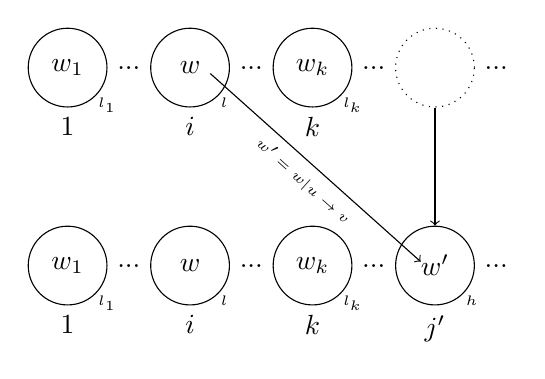
\begin{tikzpicture}
[
cell-a/.style={circle, draw, minimum size = 10mm},
cell-b/.style={circle, draw, dotted, minimum size = 10mm},
text-a/.style={}
]

\node (cell-1)     [cell-a]                                 {$w_1$};
\node (cell-1-id)  [text-a, below       =  0.0cm of cell-1] {$1$};
\node (cell-1-lb)  [text-a, below right = -1.3mm of cell-1] {\tiny $l_1$};
\node (dots-1)     [text-a, right       =  0.0mm of cell-1] {$...$};
\node (cell-i)     [cell-a,right        =  0.0mm of dots-1] {$w$};
\node (cell-i-id)  [text-a, below       =  0.0cm of cell-i] {$i$};
\node (cell-i-lb)  [text-a, below right = -1.3mm of cell-i] {\tiny $l$};
\node (dots-2)     [text-a, right       =  0.0mm of cell-i] {$...$};
\node (cell-k)     [cell-a,right        =  0.0mm of dots-2] {$w_k$};
\node (cell-k-id)  [text-a, below       =  0.0cm of cell-k] {$k$};
\node (cell-k-lb)  [text-a, below right = -1.3mm of cell-k] {\tiny $l_k$};
\node (dots-3)     [text-a, right       =  0.0cm of cell-k] {$...$};
\node (cell-vt)    [cell-b, right       =  0.0mm of dots-3] {};
\node (dots-4)     [text-a, right       =  0.0mm of cell-vt] {$...$};
\node (cell-12)    [cell-a, below       =  1.5cm of cell-1]   {$w_1$};
\node (cell-12-id) [text-a, below       =  0.0cm of cell-12] {$1$};
\node (l1)         [text-a, below right = -1.3mm of cell-12] {\tiny $l_1$};
\node (dots-12)    [text-a, right       =  0.0mm of cell-12] {$...$};
\node (cell-i2)    [cell-a, right       =  0.0mm of dots-12] {$w$};
\node (cell-i2-id) [text-a, below       =  0.0cm of cell-i2] {$i$};
\node (cell-i2-lb) [text-a, below right = -1.3mm of cell-i2] {\tiny $l$};
\node (dots-22)    [text-a, right       =  0.0mm of cell-i2] {$...$};
\node (cell-k2)    [cell-a,right        =  0.0mm of dots-22] {$w_k$};
\node (cell-k2-id) [text-a, below       =  0.0cm of cell-k2] {$k$};
\node (cell-k2-lb) [text-a, below right = -1.3mm of cell-k2] {\tiny $l_k$};
\node (dots-32)    [text-a, right       =  0.0mm of cell-k2] {$...$};
\node (cell-j')    [cell-a, right       =  0.0mm of dots-32] {$w'$};
\node (cell-j'-id) [text-a, below       =  0.0cm of cell-j'] {$j'$};
\node (cell-j'-lb) [text-a, below right = -1.3mm of cell-j'] {\tiny $h$};
\node (w)          [circle, minimum size = 0.5cm] at (cell-i.base){}; 
\node (w')         [circle, minimum size = 0.5cm] at (cell-j'.base) {};
\node (dots-33)    [text-a, right       =  0.0mm of cell-j'] {$...$};
\draw [ ->] (cell-vt) -- (cell-j');
\draw [->] (w.east) -- (w'.north west) node[midway, sloped, below] {\tiny $w'= w |u \rightarrow v$} ;

\end{tikzpicture}
\end{center}
\end{figure}

\begin{itemize}
\item $j' \in \mathbb{N}'$ - primed id
\item $h \in Lab$ - label
\item $i \in \mathbb{N}'_k$ - cell id 
\item $w_1,...,w,...,w_k \in O^{\circ}$ - multisets
\item $u,v \in O^{\circ}$ - multisets
\item $(u,v)$ - written as $u \rightarrow v$
\end{itemize}

% ================================================================================================ %

\item $Change\mn Relation$
\begin{itemize}
\item $Change\mn Relation$ is a \textit{graph transducer} that updates the relation $\rho$.
\item This transducer should be recursive and it can only add and remove edges.
\end{itemize}

% ================================================================================================ %

\end{enumerate}

% ================================================================================================ %

\subsection{Eligibility of an Id Vector}

% ================================================================================================ %

\begin{enumerate}

% ================================================================================================ %

\item $ID' = (id'_1,...,id'_i,...,id'_{n'}) \in \mathbb{N}^{n'}$ 

\begin{figure}[H]
\begin{center}
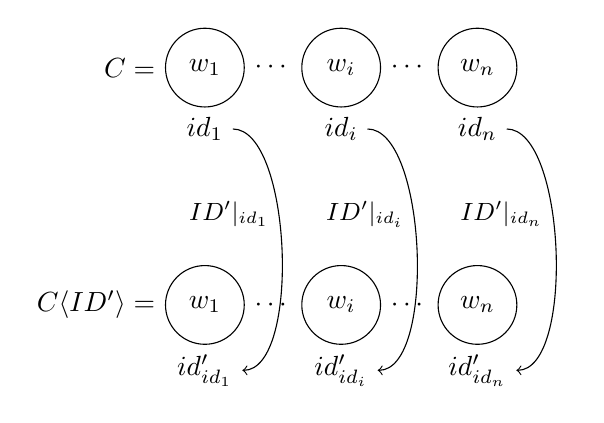
\begin{tikzpicture}
[ 
cell-a/.style={circle, draw, minimum size = 10mm},
cell-b/.style={circle, draw, minimum size = 10mm, dotted},
text-a/.style={black},
text-b/.style={blue}
]

\node (cell-1)     [cell-a]                              {$w_1$};
\node (cell-1-id)  [text-a, below =  00.00mm of cell-1]  {$id_1$};
\node (dots-1)     [text-a, right =  00.00mm of cell-1]  {$\cdots$};
\node (cell-i)     [cell-a, right =  00.00mm of dots-1]  {$w_i$};
\node (cell-i-id)  [text-a, below =  00.00mm of cell-i]  {$id_i$};
\node (dots-2)     [text-a, right =  00.00mm of cell-i]  {$\cdots$};
\node (cell-n)     [cell-a, right =  00.00mm of dots-2]  {$w_n$};
\node (cell-n-id)  [text-a, below =  00.00mm of cell-n]  {$id_n$};
\node (config)     [text-a, left  =  00.00mm of cell-1]  {$C=$};
\node (cell-1')    [cell-a, below =  20.00mm of cell-1]  {$w_1$};
\node (cell-1'-id) [text-a, below =  00.00mm of cell-1'] {$id'_{id_1}$};
\node (dots-3)     [text-a, right =  00.00mm of cell-1']  {$\cdots$};
\node (cell-i')    [cell-a, right =  00.00mm of dots-3]  {$w_i$};
\node (cell-i'-id) [text-a, below =  00.00mm of cell-i'] {$id'_{id_i}$};
\node (dots-4)     [text-a, right =  00.00mm of cell-i']  {$\cdots$};
\node (cell-n')    [cell-a, right =  00.00mm of dots-4]  {$w_n$};
\node (cell-n'-id) [text-a, below =  00.00mm of cell-n']  {$id'_{id_n}$};
\node (config')    [text-a, left  =  00.00mm of cell-1']  {$C\langle ID'\rangle=$};
\draw [->] (cell-1-id.east) .. controls +(right:07.50mm) and +(right:07.50mm) 
                            .. (cell-1'-id.east) node[pos=0.40, left] {\small $ID'|_{id_1}$};
\draw [->] (cell-i-id.east) .. controls +(right:07.50mm) and +(right:07.50mm) .. (cell-i'-id.east) node[pos=0.40, left] {\small $ID'|_{id_i}$};
\draw [->] (cell-n-id.east) .. controls +(right:07.50mm) and +(right:07.50mm) .. (cell-n'-id.east) node[pos=0.40, left] {\small $ID'|_{id_n}$};

\end{tikzpicture}
\end{center}
\end{figure}

% ================================================================================================ %

\begin{itemize}
\item $ID'|_x = id'_x$ 
\item $ID'|_{id_i} = id'_{id_i}$
\item $C = \{(id_1,w_n),...,(id_i,w_i),...(id_n,w_n)\}$
\item $C\langle ID'\rangle = \{(ID'|_{id_1},w_n),...,(ID'|_{id_i},w_i),...(ID'|_{id_n},w_n)\}$
\item $C\langle ID'\rangle = \{(id'_{id_1},w_n),...,(id'_{id_i},w_i),...(id'_{id_n},w_n)\}$
\item $|ID'| = n' = max\{id_i\}$
\item $|C| = n$
\item $|C| = n \leq n' = |ID'|$
\end{itemize}

% ================================================================================================ %

\item $Eligible(ID', r, \mathcal{C})$ 

\begin{figure}[H]
\begin{center}
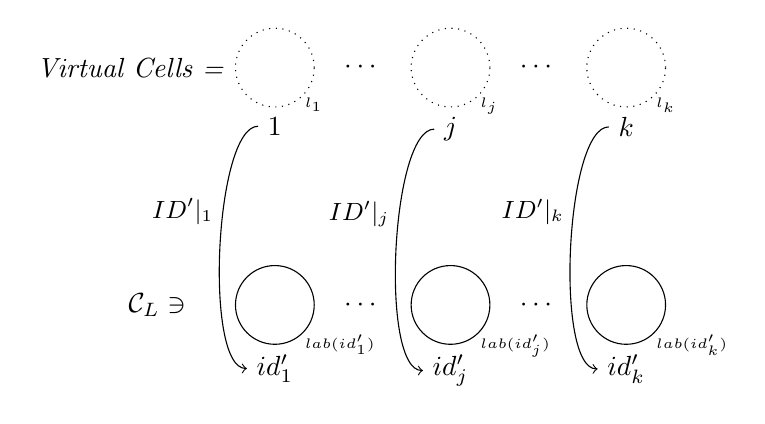
\begin{tikzpicture}
[ 
cell-a/.style={circle, draw, minimum size = 10mm},
cell-b/.style={circle, draw, minimum size = 10mm, dotted},
text-a/.style={black},
text-b/.style={blue}
]

\node (cell-1)     [cell-b]                                    {};
\node (cell-1-id)  [text-a, below       =  00.00mm of cell-1]  {$1$};
\node (cell-1-lb)  [text-a, below right = -01.40mm of cell-1]  {\tiny $l_1$}; 
\node (dots-1)     [text-a, right       =  02.50mm of cell-1]  {$\cdots$};
\node (cell-j)     [cell-b, right       =  02.50mm of dots-1]  {};
\node (cell-j-id)  [text-a, below       =  00.00mm of cell-j]  {$j$}; 
\node (cell-j-lb)  [text-a, below right = -01.40mm of cell-j]  {\tiny $l_j$}; 
\node (dots-2)     [text-a, right       =  02.50mm of cell-j]  {$\cdots$};
\node (cell-k)     [cell-b, right       =  02.50mm of dots-2]  {};
\node (cell-k-id)  [text-a, below       =  00.00mm of cell-k]  {$k$}; 
\node (cell-k-lb)  [text-a, below right = -01.40mm of cell-k]  {\tiny $l_k$}; 
\node (virt)       [text-a, left        =  00.00mm of cell-1]  {\textit{Virtual Cells =}};
\node (cell-1')    [cell-a, below       =  20.00mm of cell-1]  {};
\node (cell-1'-id) [text-a, below       =  00.00mm of cell-1'] {$id'_1$};
\node (cell-1'-lb) [text-a, below right = -01.40mm of cell-1'] {\tiny $lab(id'_1)$}; 
\node (dots-3)     [text-a, right       =  02.50mm of cell-1'] {$\cdots$};
\node (cell-j')    [cell-a, right       =  02.50mm of dots-3]  {};
\node (cell-j'-id) [text-a, below       =  00.00mm of cell-j'] {$id'_j$};
\node (cell-j'-lb) [text-a, below right = -01.40mm of cell-j'] {\tiny $lab(id'_j)$}; 
\node (dots-4)     [text-a, right       =  02.50mm of cell-j'] {$\cdots$};
\node (cell-k')    [cell-a, right       =  02.50mm of dots-4]  {};
\node (cell-k'-id) [text-a, below       =  00.00mm of cell-k'] {$id'_k$}; 
\node (cell-k'-lb) [text-a, below right = -01.40mm of cell-k'] {\tiny $lab(id'_k)$}; 
\node (CM)         [text-a, left        =  05.00mm of cell-1'] {$\mathcal{C}_L \ni$};
\draw [->] (cell-1-id.west) .. controls +(left:05.50mm) and +(left:05.50mm) .. (cell-1'-id.west) node[pos=0.40, left] {\small $ID'|_1$};
\draw [->] (cell-j-id.west) .. controls +(left:05.50mm) and +(left:05.50mm) .. (cell-j'-id.west) node[pos=0.40, left] {\small $ID'|_j$};
\draw [->] (cell-k-id.west) .. controls +(left:05.50mm) and +(left:05.50mm) .. (cell-k'-id.west) node[pos=0.40, left] {\small $ID'|_k$};

\end{tikzpicture}
\end{center}
\end{figure}

\begin{itemize}
\item $ID' = (id'_1,...,id'_j,...,id'_k) \in \mathbb{N}^k$ 
\item $r$ is a \textit{k-degree interaction rule}
\item $r \langle ID'\rangle$ - \textit{instantiated rule} - replace virtual ids with ids in $ID'$
\item $Labels(r) = (l_1,...,l_j,...,l_k)$
\item $\mathcal{C} = (L,\rho)$
\item $lab: \mathbb{N} \rightarrow Lab$
\item $Eligible(ID',r,\mathcal{C}) \Leftrightarrow$ :
\begin{itemize}
\item $\forall x,y  \in \{1,...,k\}: (x \neq y) \rightarrow (id'_x \neq id'_y)$ [id uniqueness]
\item $\forall x    \in \{1,...,k\}: l_x = lab(id'_x)$  [label consistency]
\item $\forall x,y, \in \{1,...,k\}: (x,y) \in \rho(r) \rightarrow (id'_x, id'_y) 
                                                 \in \mathcal{C}_{\rho}$ [relations consistency]
\end{itemize}
\item $\mathcal{I}_{\mathcal{C}} (r) = \{ID' \s|\s Eligible(ID',r, \mathcal{C})\}$
\end{itemize}

% ================================================================================================ %

\end{enumerate}

% ================================================================================================ %

\subsection{Applicability of a Multiset of Rules}

% ================================================================================================ %

\begin{itemize}
\item $R = \{r_1,...,r_i,...,r_n\}$ - \textit{multiset} of rules
\item $\mathcal{I}_{\mathcal{C}}(r_i) = \{ID'_{i,1},...,ID'_{i,j_i},...,ID'_{i,k_i}\}$
\item $RI = \{r_1\langle ID'_{1,j_1}\rangle,...,r_i\langle ID'_{i,j_i}\rangle,...,
            r_n\langle ID'_{n,j_n}\rangle\}$ - \textit{multiset of instantiated rules}
\end{itemize}

$applicable(RI, \mathcal{C}) \Leftrightarrow \forall r_i \in R: \mathcal{I}_{\mathcal{C}}(r_i) 
\neq \emptyset: \forall r_i\la ID'_{i,j_i}\ra \in RI:$

\begin{enumerate}
\item $\forall P \in Perm(r_i\la ID'_{i,j_i}\ra) \cup \{DP\}: P \subseteq \overline{\mathcal{C}}_L$
      \begin{itemize}
      \item $DP = \{(id_i,u)\s |\s (j', h, id_i, u \rightarrow v) \in 
            Generate\mn and\mn Copy(r_i\la ID'_{i,j_i}\ra)\}$
      \end{itemize}

% ================================================================================================ %

\begin{figure}[H]
\begin{center}
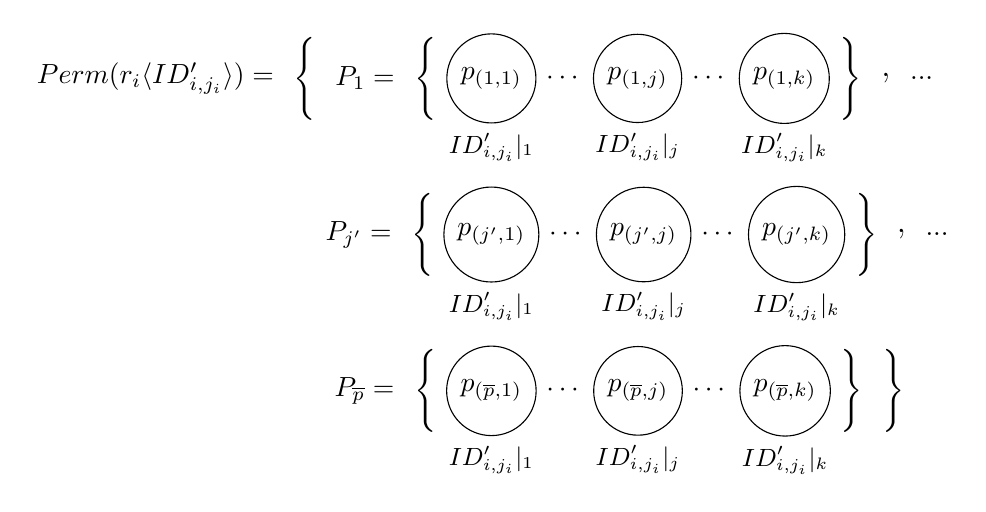
\begin{tikzpicture}
[
cell-a/.style={circle, draw, minimum size = 10mm},
cell-b/.style={circle, draw, minimum size = 10mm, dotted},
text-a/.style={black}
]
\node (cell-11)    [cell-a]                              {$p_{(1,1)}$};
\node (cell-11-id) [text-a, below =  00.00mm of cell-11] {\small $ID'_{i,j_i}|_1$};
\node (dots-1)     [text-a, right =  00.00mm of cell-11] {$\cdots$};
\node (cell-1j)    [cell-a, right =  00.00mm of dots-1 ] {$p_{(1,j)}$};
\node (cell-1j-id) [text-a, below =  00.00mm of cell-1j] {\small $ID'_{i,j_i}|_j$};
\node (dots-2)     [text-a, right =  00.00mm of cell-1j] {$\cdots$};
\node (cell-1k)    [cell-a, right =  00.00mm of dots-2 ] {$p_{(1,k)}$};
\node (cell-1k-id) [text-a, below =  00.00mm of cell-1k] {\small $ID'_{i,j_i}|_k$};
\node (brac-11)    [text-a, left  =  00.00mm of cell-11] {$\Bigg\{$};
\node (brac-12)    [text-a, right =  00.00mm of cell-1k] {$\Bigg\}$};
\node (P1)         [text-a, left  =  00.00mm of brac-11] {$P_1=$};
\node (coma1)      [text-a, right =  00.00mm of brac-12] {\large $,$};
\node (brac-01)    [text-a, left  =  00.00mm of P1     ] {$\Bigg\{$};
\node (dots-0')    [text-a, right =  00.00mm of coma1  ] {$...$};
\node (cell-j1)    [cell-a, below =  08.00mm of cell-11] {$p_{(j',1)}$};
\node (cell-j1-id) [text-a, below =  00.00mm of cell-j1] {\small $ID'_{i,j_i}|_1$};
\node (dots-3)     [text-a, right =  00.00mm of cell-j1] {$\cdots$};
\node (cell-jj)    [cell-a, right =  00.00mm of dots-3 ] {$p_{(j',j)}$};
\node (cell-jj-id) [text-a, below =  00.00mm of cell-jj] {\small $ID'_{i,j_i}|_j$};
\node (dots-3)     [text-a, right =  00.00mm of cell-jj] {$\cdots$};
\node (cell-jk)    [cell-a, right =  00.00mm of dots-3 ] {$p_{(j',k)}$};
\node (cell-jk-id) [text-a, below =  00.00mm of cell-jk] {\small $ID'_{i,j_i}|_k$};
\node (brac-j1)    [text-a, left  =  00.00mm of cell-j1] {$\Bigg\{$};
\node (brac-j2)    [text-a, right =  00.00mm of cell-jk] {$\Bigg\}$};
\node (PJ)         [text-a, left  =  00.00mm of brac-j1] {$P_{j'}=$};
\node (coma2)      [text-a, right =  00.00mm of brac-j2] {\large $,$};
\node (dots-1')    [text-a, right =  00.00mm of coma2  ] {$...$};
\node (cell-p1)    [cell-a, below =  08.00mm of cell-j1] {$p_{(\overline{p},1)}$};
\node (cell-p1-d)  [text-a, below =  00.00mm of cell-p1] {\small $ID'_{i,j_i}|_1$};
\node (dots-4)     [text-a, right =  00.00mm of cell-p1] {$\cdots$};
\node (cell-pj)    [cell-a, right =  00.00mm of dots-4 ] {$p_{(\overline{p},j)}$};
\node (cell-pj-id) [text-a, below =  00.00mm of cell-pj] {\small $ID'_{i,j_i}|_j$};
\node (dots-4)     [text-a, right =  00.00mm of cell-pj] {$\cdots$};
\node (cell-pk)    [cell-a, right =  00.00mm of dots-4 ] {$p_{(\overline{p},k)}$};
\node (cell-pk-id) [text-a, below =  00.00mm of cell-pk] {\small $ID'_{i,j_i}|_k$};
\node (brac-p1)    [text-a, left  =  00.00mm of cell-p1] {$\Bigg\{$};
\node (brac-p2)    [text-a, right =  00.00mm of cell-pk] {$\Bigg\}$};
\node (PP)         [text-a, left  =  00.00mm of brac-p1] {$P_{\overline{p}}=$};
\node (brac-02)    [text-a, right =  00.00mm of brac-p2] {$\Bigg\}$};
\node (Perm)       [text-a, left  =  00.00mm of brac-01] {$Perm(r_i\la ID'_{i,j_i}\ra)=$};
\end{tikzpicture}
\end{center}
\end{figure}

% ================================================================================================ %

\begin{figure}[H]
\begin{center}
\begin{tikzpicture}
[ 
cell-a/.style={circle, draw, minimum size =  10.00mm},
text-a/.style={black}
]
\node (dots-1)    [text-a, left  =  00.00mm of cell-i] {$\cdots$};
\node (cell-i)    [cell-a, right =  00.00mm of dots-1] {$u$};
\node (cell-i-id) [text-a, below =  00.00mm of cell-i] {$id_i$};
\node (dots-2)    [text-a, right =  00.00mm of cell-i] {$\cdots$};
\node (brac-1)    [text-a, left  =  00.00mm of dots-1] {$\Bigg\{$};
\node (brac-2)    [text-a, right =  00.00mm of dots-2] {$\Bigg\}$};
\node (DP)        [text-a, left  =  00.00mm of brac-1] {$DP=$};
\end{tikzpicture}
\end{center}
\end{figure}

% ================================================================================================ %

\begin{figure}[H]
\begin{center}
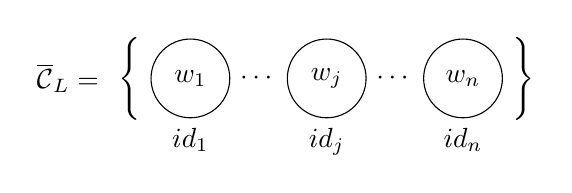
\begin{tikzpicture}
[ 
cell-a/.style={circle, draw, minimum size =  10.00mm},
text-a/.style={black}
]
\node (cell-1)    [cell-a                            ] {$w_1$};
\node (cell-1-id) [text-a, below =  00.00mm of cell-1] {$id_1$};
\node (dots-1)    [text-a, right =  00.00mm of cell-1] {$\cdots$};
\node (cell-j)    [cell-a, right =  00.00mm of dots-1] {$w_j$};
\node (cell-j-id) [text-a, below =  00.00mm of cell-j] {$id_j$};
\node (dots-2)    [text-a, right =  00.00mm of cell-j] {$\cdots$};
\node (cell-n)    [cell-a, right =  00.00mm of dots-2] {$w_n$};
\node (cell-n-id) [text-a, below =  00.00mm of cell-n] {$id_n$};
\node (brac-1)    [text-a, left  =  00.00mm of cell-1] {$\Bigg\{$};
\node (brac-2)    [text-a, right =  00.00mm of cell-n] {$\Bigg\}$};
\node (C)         [text-a, left  =  00.00mm of brac-1] {$\overline{\mathcal{C}}_L=$};
\end{tikzpicture}
\end{center}
\end{figure}

% ================================================================================================ %

\item $\forall F \in For(r_i\la ID'_{i,j_i}\ra): F \subseteq \overline{\mathcal{C}}_L$

\begin{figure}[H]
\begin{center}
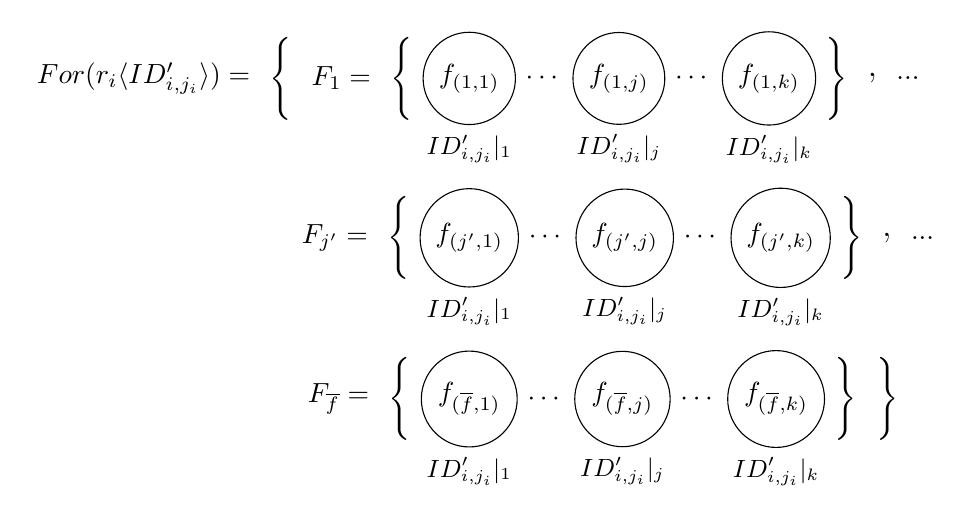
\begin{tikzpicture}
[
cell-a/.style={circle, draw, minimum size = 10mm},
cell-b/.style={circle, draw, minimum size = 10mm, dotted},
text-a/.style={black}
]
\node (cell-11)    [cell-a]                              {$f_{(1,1)}$};
\node (cell-11-id) [text-a, below =  00.00mm of cell-11] {\small $ID'_{i,j_i}|_1$};
\node (dots-1)     [text-a, right =  00.00mm of cell-11] {$\cdots$};
\node (cell-1j)    [cell-a, right =  00.00mm of dots-1 ] {$f_{(1,j)}$};
\node (cell-1j-id) [text-a, below =  00.00mm of cell-1j] {\small $ID'_{i,j_i}|_j$};
\node (dots-2)     [text-a, right =  00.00mm of cell-1j] {$\cdots$};
\node (cell-1k)    [cell-a, right =  00.00mm of dots-2 ] {$f_{(1,k)}$};
\node (cell-1k-id) [text-a, below =  00.00mm of cell-1k] {\small $ID'_{i,j_i}|_k$};
\node (brac-11)    [text-a, left  =  00.00mm of cell-11] {$\Bigg\{$};
\node (brac-12)    [text-a, right =  00.00mm of cell-1k] {$\Bigg\}$};
\node (F1)         [text-a, left  =  00.00mm of brac-11] {$F_1=$};
\node (coma1)      [text-a, right =  00.00mm of brac-12] {\large $,$};
\node (brac-01)    [text-a, left  =  00.00mm of F1     ] {$\Bigg\{$};
\node (dots-0')    [text-a, right =  00.00mm of coma1  ] {$...$};
\node (cell-j1)    [cell-a, below =  08.00mm of cell-11] {$f_{(j',1)}$};
\node (cell-j1-id) [text-a, below =  00.00mm of cell-j1] {\small $ID'_{i,j_i}|_1$};
\node (dots-3)     [text-a, right =  00.00mm of cell-j1] {$\cdots$};
\node (cell-jj)    [cell-a, right =  00.00mm of dots-3 ] {$f_{(j',j)}$};
\node (cell-jj-id) [text-a, below =  00.00mm of cell-jj] {\small $ID'_{i,j_i}|_j$};
\node (dots-3)     [text-a, right =  00.00mm of cell-jj] {$\cdots$};
\node (cell-jk)    [cell-a, right =  00.00mm of dots-3 ] {$f_{(j',k)}$};
\node (cell-jk-id) [text-a, below =  00.00mm of cell-jk] {\small $ID'_{i,j_i}|_k$};
\node (brac-j1)    [text-a, left  =  00.00mm of cell-j1] {$\Bigg\{$};
\node (brac-j2)    [text-a, right =  00.00mm of cell-jk] {$\Bigg\}$};
\node (FJ)         [text-a, left  =  00.00mm of brac-j1] {$F_{j'}=$};
\node (coma2)      [text-a, right =  00.00mm of brac-j2] {\large $,$};
\node (dots-1')    [text-a, right =  00.00mm of coma2  ] {$...$};
\node (cell-f1)    [cell-a, below =  08.00mm of cell-j1] {$f_{(\overline{f},1)}$};
\node (cell-f1-d)  [text-a, below =  00.00mm of cell-f1] {\small $ID'_{i,j_i}|_1$};
\node (dots-4)     [text-a, right =  00.00mm of cell-f1] {$\cdots$};
\node (cell-fj)    [cell-a, right =  00.00mm of dots-4 ] {$f_{(\overline{f},j)}$};
\node (cell-fj-id) [text-a, below =  00.00mm of cell-fj] {\small $ID'_{i,j_i}|_j$};
\node (dots-4)     [text-a, right =  00.00mm of cell-fj] {$\cdots$};
\node (cell-fk)    [cell-a, right =  00.00mm of dots-4 ] {$f_{(\overline{f},k)}$};
\node (cell-fk-id) [text-a, below =  00.00mm of cell-fk] {\small $ID'_{i,j_i}|_k$};
\node (brac-f1)    [text-a, left  =  00.00mm of cell-f1] {$\Bigg\{$};
\node (brac-f2)    [text-a, right =  00.00mm of cell-fk] {$\Bigg\}$};
\node (FF)         [text-a, left  =  00.00mm of brac-f1] {$F_{\overline{f}}=$};
\node (brac-02)    [text-a, right =  00.00mm of brac-f2] {$\Bigg\}$};
\node (For)        [text-a, left  =  00.00mm of brac-01] {$For(r_i\la ID'_{i,j_i}\ra)=$};
\end{tikzpicture}
\end{center}
\end{figure}

% ================================================================================================ %

\item $\big(\bigcup_{i=1}^{n} U_i \big) \subseteq \overline{\mathcal{C}}_L$
       \begin{itemize}
       \item $Rewrite(r\la ID'_{i,j_i}\ra) = U_i \rightarrow V_i$
       \item $U_i,V_i \in \mathbb{C}$
       \end{itemize}

\begin{figure}[H]
\begin{center}
\begin{tikzpicture}
[ 
cell-a/.style={circle, draw, minimum size =  10.00mm},
text-a/.style={black}
]
\node (dots-1)    [text-a, left  =  00.00mm of cell-i] {$\cdots,$};
\node (cell-i)    [cell-a, right =  00.00mm of dots-1] {$u$};
\node (cell-i-id) [text-a, below =  00.00mm of cell-i] {$id_j$};
\node (dots-2)    [text-a, right =  00.00mm of cell-i] {$,\cdots$};
\node (brac-1)    [text-a, left  =  00.00mm of dots-1] {$\Bigg\{$};
\node (brac-2)    [text-a, right =  00.00mm of dots-2] {$\Bigg\}$};
\node (U)         [text-a, left  =  00.00mm of brac-1] {$U_i=$};
\end{tikzpicture}
\end{center}
\end{figure}

\item $\forall id_s, i,k: \s [(id_s, l)  \in Label\mn Rename(r_i \la ID'_{i,j_i} \ra)\s \land 
      \s (id_s, l') \in Label\mn Rename(r_k \la ID'_{k,j_k} \ra)] \rightarrow l = l'$ 

\item $\forall i,k: Change\mn Relation(r_k)(Change\mn Relation(r_i)(\mathcal{C}_{\rho})) =  
                    Change\mn Relation(r_i)(Change\mn Relation(r_k)(\mathcal{C}_{\rho}))$ 

% ================================================================================================ %

\end{enumerate}
  
\begin{itemize} 
\item $Applicable(R,\mathcal{C}) = \{RI\s |\s applicable(RI,\mathcal{C})\}$
\item $Applicable(\Pi, \mathcal{C}) = \bigcup_{Applicable(R, \mathcal{C})\neq \emptyset} 
      Applicable(R,\mathcal{C})$
\end{itemize}

% ================================================================================================ %

\subsection{Applying a Multiset of Rules}

% ================================================================================================ %

\begin{enumerate}

% ================================================================================================ %

\item $L_1 = \{(i_1,l_1,w'_1)...(i_n,l_n,w'_n)\}$
      \begin{figure}[H]
      \begin{center}
      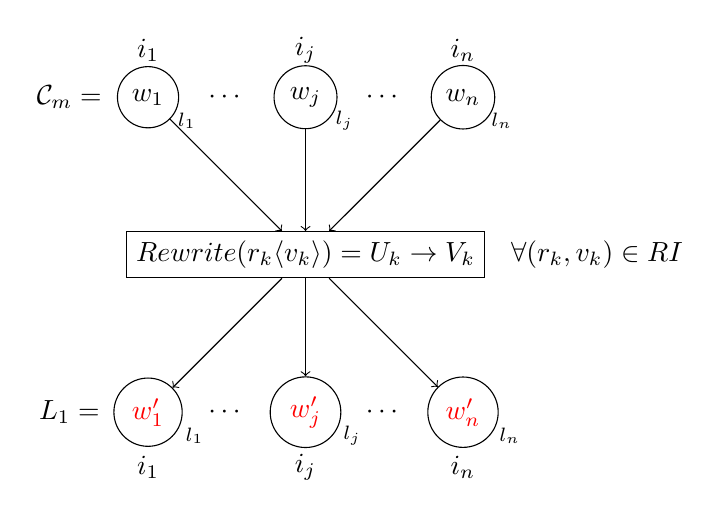
\begin{tikzpicture}[scale=1.0]
      %\draw [dotted] (-5,-5) grid (5,5); \draw [->] (0,0) -- (0,5); \draw [->] (0,0) -- (5,0);
      \node                  (l) at (-1.0,  2.0) {$\mathcal{C}_m =$};
      \node                 (l2) at (-1.0, -2.0) {$L_1 =$};
      \node [circle, draw]  (w1) at ( 0.0,  2.0) {$w_1$};
      \node                 (i1) at ( 0.0,  2.6) {$i_1$};
      \node                 (l1) at ( 0.5,  1.7) {$_{l_1}$};
      \node                 (wx) at ( 1.0,  2.0) {$\cdots$};
      \node [circle, draw]  (wj) at ( 2.0,  2.0) {$w_j$};
      \node                 (ij) at ( 2.0,  2.6) {$i_j$};
      \node                 (lj) at ( 2.5,  1.7) {$_{l_j}$};
      \node                 (wy) at ( 3.0,  2.0) {$\cdots$};
      \node [circle, draw]  (wn) at ( 4.0,  2.0) {$w_n$};
      \node                 (in) at ( 4.0,  2.6) {$i_n$};
      \node                 (ln) at ( 4.5,  1.7) {$_{l_n}$};
      \node [circle, draw]  (w12) at ( 0.0, -2.0) {\textcolor{red}{$w'_1$}};
      \node                 (i12) at ( 0.0, -2.7) {$i_1$};
      \node                 (l12) at ( 0.6, -2.3) {$_{l_1}$};
      \node                 (wx2) at ( 1.0, -2.0) {$\cdots$};
      \node [circle, draw]  (wj2) at ( 2.0, -2.0) {\textcolor{red}{$w'_j$}};
      \node                 (ij2) at ( 2.0, -2.7) {$i_j$};
      \node                 (lj2) at ( 2.6, -2.3) {$_{l_j}$};
      \node                 (wy2) at ( 3.0, -2.0) {$\cdots$};
      \node [circle, draw]  (wn2) at ( 4.0, -2.0) {\textcolor{red}{$w'_n$}};
      \node                 (in2) at ( 4.0, -2.7) {$i_n$};
      \node                 (ln2) at ( 4.6, -2.3) {$_{l_n}$};
      \node [rectangle, draw]  (rk) at ( 2.0,  0.0) {$Rewrite(r_k\langle v_k \rangle)= U_k \rightarrow V_k$};
      \node                   (rk2) at ( 5.7,  0.0) {$\forall (r_k,v_k) \in RI$};
      \draw [->] (w1) -- (rk);
      \draw [->] (wj) -- (rk);
      \draw [->] (wn) -- (rk);
      \draw [->] (rk) -- (w12);
      \draw [->] (rk) -- (wj2);
      \draw [->] (rk) -- (wn2);
      \end{tikzpicture}
      \end{center}
      \end{figure}
         \begin{itemize}
         \item $$w'_j = w_j - \Bigg(\bigcup_{(r_k,v_k)\in RI} U_k |_j \Bigg) + \Bigg(\bigcup_{(r_k,v_k) \in RI } V_k|_j \Bigg)$$
         \item $RI = \{(r_1,v_1)...(r_n,v_n)\}$
         \item $\mathcal{C} = (\{(i_1,l_1,w_1)...(i_n,l_n,w_n)\},\rho)$ 
         \item $Rewrite(r_k\langle v_k \rangle) = U_k \rightarrow V_k$
         \item $U_k,V_k \in \mathbb{C}_k$
         \end{itemize}
% ================================================================================================ %

\item $L_2 = \{(i_1,l'_1,w'_1)...(i_n,l'_n,w'_n)\}$
      \begin{figure}[H]
      \begin{center}
      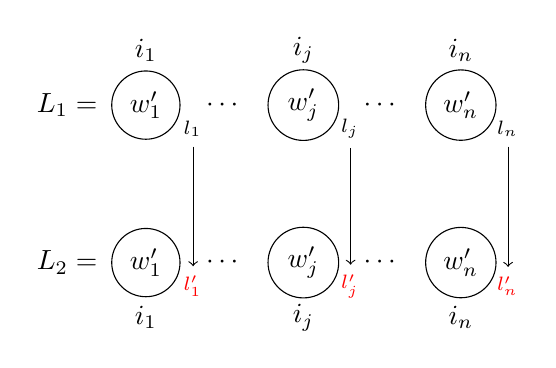
\begin{tikzpicture}[scale=1.0]
      %\draw [dotted] (-5,-5) grid (5,5); \draw [->] (0,0) -- (0,5); \draw [->] (0,0) -- (5,0);
      \node                  (l) at (-1.0,  2.0) {$ L_1 =$};
      \node                  (l) at (-1.0,  0.0) {$ L_2 =$};
      \node [circle, draw]  (w1) at ( 0.0,  2.0) {$w'_1$};
      \node                 (i1) at ( 0.0,  2.7) {$i_1$};
      \node                 (l1) at ( 0.6,  1.7) {$_{l_1}$};
      \node                 (wx) at ( 1.0,  2.0) {$\cdots$};
      \node [circle, draw]  (wj) at ( 2.0,  2.0) {$w'_j$};
      \node                 (ij) at ( 2.0,  2.7) {$i_j$};
      \node                 (lj) at ( 2.6,  1.7) {$_{l_j}$};
      \node                 (wy) at ( 3.0,  2.0) {$\cdots$};
      \node [circle, draw]  (wn) at ( 4.0,  2.0) {$w'_n$};
      \node                 (in) at ( 4.0,  2.7) {$i_n$};
      \node                 (ln) at ( 4.6,  1.7) {$_{l_n}$};
      \node [circle, draw]  (w12) at ( 0.0,  0.0) {$w'_1$};
      \node                 (i12) at ( 0.0, -0.7) {$i_1$};
      \node                 (l12) at ( 0.6, -0.3) {\textcolor{red}{$_{l'_1}$}};
      \node                 (wx2) at ( 1.0,  0.0) {$\cdots$};
      \node [circle, draw]  (wj2) at ( 2.0,  0.0) {$w'_j$};
      \node                 (ij2) at ( 2.0, -0.7) {$i_j$};
      \node                 (lj2) at ( 2.6, -0.3) {\textcolor{red}{$_{l'_j}$}};
      \node                 (wy2) at ( 3.0, -0.0) {$\cdots$};
      \node [circle, draw]  (wn2) at ( 4.0, -0.0) {$w'_n$};
      \node                 (in2) at ( 4.0, -0.7) {$i_n$};
      \node                 (ln2) at ( 4.6, -0.3) {\textcolor{red}{$_{l'_n}$}};
      \draw [->] (l1) -- (l12);
      \draw [->] (lj) -- (lj2);
      \draw [->] (ln) -- (ln2);
      \end{tikzpicture}
      \end{center}
      \end{figure}
         \begin{itemize}
         \item \[ l'_j = \begin{cases} 
                         e_s, & \text{if } \exists(r_k,v_k)\in RI \text{ such that } (j,e_s) \in Label\mn Rename(r_k\langle v_k\rangle)\\
                         l_j, & \text{otherwise} 
                         \end{cases}\] 
        \end{itemize}
% ================================================================================================ %
   \item $L_c = L_c(r_1) \cdot \cdots \cdot L_c(r_n)$
      \begin{figure}[H]
      \begin{center}
      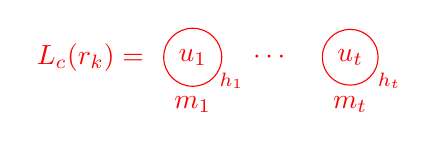
\begin{tikzpicture}[scale=1.0]
      %\draw [dotted] (-2,-2) grid (10,5); \draw [->] (0,0) -- (0,5); \draw [->] (0,0) -- (10,0);
      \textcolor{red}{
      \node                  (l) at (-1.3,  2.0) {$ L_c(r_k) =$};
      \node [circle, draw]  (u1) at ( 0.0,  2.0) {$u_1$};
      \node                 (m1) at ( 0.0,  1.4) {$m_1$};
      \node                 (h1) at ( 0.5,  1.7) {$_{h_1}$};
      \node                (dt1) at ( 1.0,  2.0) {$\cdots$};
      \node [circle, draw]  (ut) at ( 2.0,  2.0) {$u_t$};
      \node                 (mt) at ( 2.0,  1.4) {$m_t$};
      \node                 (ht) at ( 2.5,  1.7) {$_{h_t}$};}
      \end{tikzpicture}
      \end{center}
      \end{figure}
         \begin{itemize}
         \item $L_c(r_k) = \{(m_1, h_1, u_1)\cdots (m_t,h_t,u_t)\}$
         \item $Generate(r_k) = \{(1', h_1, u_1) \cdots (t', h_t, u_t)\}$
         \end{itemize}
% ================================================================================================ %
   \item $L'_c = L'_c(r_1)\cdot \cdots \cdot L'_c(r_n)$
      \begin{figure}[H]
      \begin{center}
      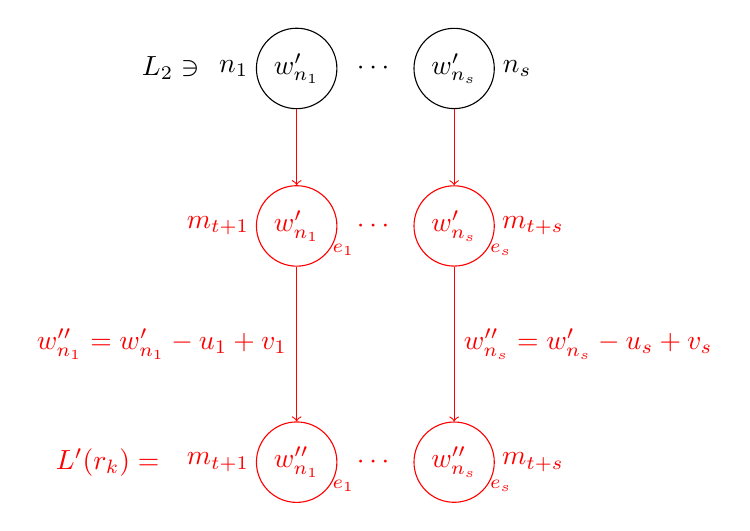
\begin{tikzpicture}[scale=1.0]
      %\draw [dotted] (-5,-5) grid (5,5); \draw [->] (0,0) -- (0,5); \draw [->] (0,0) -- (5,0);
      \node                  (l) at (-1.6,  2.0) {$ L_2 \ni$};
      \node [circle, draw]  (wn1) at ( 0.0,  2.0) {$w'_{n_1}$};
      \node                 (e1) at (-0.8,  2.0) {$n_1$};
      \node                 (wx) at ( 1.0,  2.0) {$\cdots$};
      \node [circle, draw]  (wns) at ( 2.0,  2.0) {$w'_{n_s}$};
      \node                 (ij) at ( 2.8,  2.0) {$n_s$};
      \textcolor{red}{
      \node [circle, draw]  (wn12) at ( 0.0,  0.0) {$w'_{n_1}$};
      \node                  (mt1) at (-1.0,  0.0) {$m_{t+1}$};
      \node                 (dots) at ( 1.0,  0.0) {$\cdots$};
      \node                   (e1) at ( 0.6, -0.3) {$_{e_1}$};
      \node [circle, draw]  (wns2) at ( 2.0,  0.0) {$w'_{n_s}$};
      \node                  (mts) at ( 3.0,  0.0) {$m_{t+s}$};
      \node                   (es) at ( 2.6, -0.3) {$_{e_s}$};
      \node [circle, draw]  (wn13) at ( 0.0, -3.0) {$w''_{n_1}$};
      \node                  (mt1) at (-1.0, -3.0) {$m_{t+1}$};
      \node                 (dots) at ( 1.0, -3.0) {$\cdots$};
      \node                   (e1) at ( 0.6, -3.3) {$_{e_1}$};
      \node [circle, draw]  (wns3) at ( 2.0, -3.0) {$w''_{n_s}$};
      \node                  (mts) at ( 3.0, -3.0) {$m_{t+s}$};
      \node                   (es) at ( 2.6, -3.3) {$_{e_s}$};
      \node                   (lc) at (-2.4, -3.0) {$L'(r_k) =$};
      \draw [->] (wn1) -- (wn12);
      \draw [->] (wns) -- (wns2);
      \draw [->] (wn12) -- (wn13) node[pos=0.5,left] {$w''_{n_1} = w'_{n_1} -u_1+v_1$};
      \draw [->] (wns2) -- (wns3) node[pos=0.5,right] {$w''_{n_s} = w'_{n_s}-u_s+v_s$};
      }
      \end{tikzpicture}
      \end{center}
      \end{figure}
         \begin{itemize}
         \item $L'_c(r_k) = \{(m_{t+1},e_1, w'_{n_1} - u_1 + v_1)...(m_{t+s}, e_s, w'_{n_s} - u_s + v_s)\}$
         \item $Generate\mn and \mn Copy(r_k) = \{(1',e_1, n_1, u_1 \rightarrow v_1)...(s', e_s, n_s, u_s \rightarrow v_s)\}$
         \item $(i_j, l'_j, w'_j) \in L_2$
         \end{itemize}
   \item $L_3 = L_2 \cdot  L_c \cdot L_c'$
   \item $L_4 = \{(i_1, l_1', w_1'') \cdots (i_n, l_n', w_n'')\}$
         \begin{itemize}
         \item $$w_j'' = w_j' + \Bigg(\bigcup_{\text{last}(i_k)=i_j} w_k' \Bigg)$$
         \item $(i_j, l_j', w_j') \in L_3$
         \item $\textbf{p} = (p_1,...,p_j,...,p_n)$ - vector of ``destination" cell ids for multisets from cells that may be deleted.
         \item $p_j = p(i_j)$ - destination cell for multiset from cell $i_j$. 
         \item \[ p(i_j) = \begin{cases} 
                           *  , & \text{if } \exists(r_k,v_k)\in RI \text{ such that } i_j \in Delete(r_k\langle v_k\rangle)\\
                           e  , & \text{if } \exists(r_k,v_k)\in RI \text{ such that } (i_j,e) \in Delete\mn and\mn Move(r_k\langle v_k\rangle)\\
                           i_j, & \text{otherwise} 
                           \end{cases}\] 
         \item $Delete(r) \in \mathbb{N}_k^*$ is the list of cell ids to be deleted.
         \item $Delete\mn and\mn Move(r) \in (\mathbb{N}_k \times \mathbb{N}_k)^*$. $(i,j) \in Delete\mn and\mn Move(r)$ means to delete cell $i$ and move its multiset to
               cell $j$.
         \item If $p_k = p(i_k) = i_k$, then cell $i_k$ will not be deleted.
         \item If $p_k = p(i_k) \neq i_k$ (either $p(i_k)= *$ or $p(i_k)=e$), then cell $i_k$ will be deleted.
         \item If $p_k = i_k$, then there is a sequence $x_1,...,x_{j-1},...,x_m$ of cell ids where:
               \begin{itemize}
                  \item $x_1 = p_k$
                  \item $x_j = p(x_{j-1})$ for $2 \leq j \leq m$
                  \item $x_m = z$ 
               \end{itemize}
               There is a chain of ``delete-and-move" and $z$ is the last cell id to not be deleted or to be deleted and not moved.
         \item $last(i_j) = z$
         \end{itemize}
   \item $L_5 = \{(i_1,l_1',w_1'')...(i_{n_1},l_{n_1}',w_{n_1}'')\}$ where $(i_j,l_j',w_j'') \in L_4$ and $p_j = i_j$. 
         \begin{itemize}
         \item $L_5$ contains $L_4$ cells with the deleted cells removed.
         \end{itemize}
   \item $Apply(RI,\mathcal{C}) = (L_2, \mathcal{C}_{\rho}')$
         \begin{itemize}
         \item $\mathcal{C}_{\rho}'$ is the updated `parent' relation after $CREATE\mn NODES$, $DELETE\mn NODES$, and\\ $Change\mn Relation(r_k\langle v_k\rangle)$ have been computed
               for all $(r_k,v_k) \in RI$ on $\mathcal{C}_{\rho}$.
         \end{itemize}
\end{enumerate}

\end{document}

































